\section[Leistungsaufnahme]{Leistungsaufnahme verschiedener elektronischer Bauteile}
In diesem Kapitel werden  drei verschiedene Schaltungen behandelt (vgl. Abb. \ref{fig:Leistungsaufnahme}):
\begin{itemize}
	\item Zuerst wird für Schaltung a) der Zusammenhang zwischen Strom, Spannung und Leistung untersucht.
	\item Im zweiten Teil wird für Schaltung b) der Betrag des Phasenwinkels~$|\phi|$, der Wirkwiderstand~$R_W$ sowie die Induktivität~$L$ einer Spule	 berechnet.
	\item Zuletzt wird mit den Ergebnissen aus dem zweiten Teil die Kapazität $C$ dreier, in Reihe geschalteter Kondensatoren nach Schaltung c) bestimmt, diese werden im Folgenden als ein Kondensator betrachtet.
\end{itemize}


\begin{figure}[h]
	\centering
	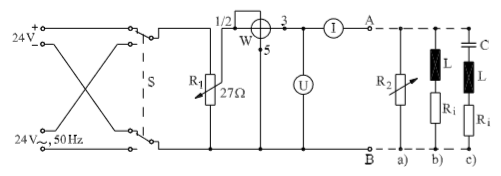
\includegraphics[width=0.9\textwidth]{res/Schaltskizze.png}
	\caption{Schaltskizze, die die im zweiten Teil des Protokolls behandelten Schaltungen beschreibt.\cite{lw}}
	\label{fig:Leistungsaufnahme}
\end{figure}

\subsection{Methoden}\label{kap:MethodenS}
Es werden in einer Schaltung gemäß Position a) in \cref{fig:Leistungsaufnahme} Leistung und Stromstärke bezüglich des Widerstandes $R_2$ bei fünf verschiedenen Spannungen bei Gleich- und Wechselstrom gemessen.
Anschließend wird der Zusammenhang zwischen der Spannung $U$ und der Stromstärke $I$, welcher mithilfe des Widerstandes definiert ist, untersucht.
Der Zusammenhang zwischen Leistung $P$ und dem Produkt aus Spannung und Stromstärke $UI$ wurde in \cref{fig:leistung-r2} graphisch dargestellt.
Um die im zweiten Teil genannten Größen zu berechnen wurde die Spannung $U$, der Strom $I$ und die Leistung $P$ gemessen. 
Die Spannung und der Strom wurden sowohl bei Wechselstrom, als auch bei Gleichstrom bestimmt, während die Leistung nur bei Wechselstrom gemessen wurde. Zu beachten ist, dass es sich bei allen im weiteren genannten Werte für $U$, $I$, die bei Wechselstrom gemessen wurden, um Effektivwerte handelt und $P$ nur gemittelt angegeben werden kann.
Im letzten Teil werden die Werte für die Induktivität und den Innenwiderstand aus dem zweiten Teil übernommen und zusätzlich wurde die Spannung, der Strom und die Leistung bei Wechselstrom aufgenommen.
Die Messungen wurden mit einem Multimeter, einem Ampermeter und einem Wattmeter durchgeführt.
All diese Messgeräte waren mit einem analogen Skala versehen. Aus diesem Grund sind alle Unsicherheiten der Messwerte, durch eine Dreiecksverteilung abzuschätzen. 
%Hier wird noch gesagt was für Unsicherheiten wird genau für die Skalen annehmen.
